\documentclass[graybox]{svmult}

% Springer fonts and formatting
\usepackage{mathptmx}       % selects Times Roman as basic font
\usepackage{helvet}         % selects Helvetica as sans-serif font
\usepackage{courier}        % selects Courier as typewriter font
\usepackage{type1cm}        % activate if fonts are not available on system

\usepackage{makeidx}         % allows index generation
\usepackage{graphicx}        % standard LaTeX graphics tool
\usepackage{multicol}        % used for the two-column index
\usepackage[bottom]{footmisc}% places footnotes at page bottom

\usepackage{amsmath,amssymb,amsfonts}
\usepackage{booktabs}
\usepackage[hidelinks]{hyperref}
\usepackage{microtype}
\usepackage{xcolor}

% Custom macros and notations
\IfFileExists{paper/macros.tex}{%
  % Reliance-Utility Benchmark Macros and Math Notation

% Number verification macro: \checknum{value}{model:corruption:column}
% Expands to the value in LaTeX, and is verified by scripts/check_numbers.py
\newcommand{\checknum}[2]{#1}

% Placeholder macro for pending empirical results
\newcommand{\TODO}[1]{\textcolor{red}{[\textbf{TODO}: #1]}}

% Common notation macros
\newcommand{\utility}{U(S)}
\newcommand{\reliance}{R(S)}
\newcommand{\normreliance}{\hat{R}(S)}
\newcommand{\crossing}{S^*}
\newcommand{\mi}{\text{MI}}
\newcommand{\jsd}{\text{JSD}}
\newcommand{\dkl}{D_{\text{KL}}}

% Table formatting macro for single-column LNCS layout
\newcommand{\fittable}[1]{\begingroup\small\setlength{\tabcolsep}{4pt}
\resizebox{\linewidth}{!}{#1}\endgroup}

% Abstract keywords macro
\providecommand{\keywords}[1]{\vspace{0.5em}\noindent\textbf{Keywords:} #1}
%
}{%
  % Reliance-Utility Benchmark Macros and Math Notation

% Number verification macro: \checknum{value}{model:corruption:column}
% Expands to the value in LaTeX, and is verified by scripts/check_numbers.py
\newcommand{\checknum}[2]{#1}

% Placeholder macro for pending empirical results
\newcommand{\TODO}[1]{\textcolor{red}{[\textbf{TODO}: #1]}}

% Common notation macros
\newcommand{\utility}{U(S)}
\newcommand{\reliance}{R(S)}
\newcommand{\normreliance}{\hat{R}(S)}
\newcommand{\crossing}{S^*}
\newcommand{\mi}{\text{MI}}
\newcommand{\jsd}{\text{JSD}}
\newcommand{\dkl}{D_{\text{KL}}}

% Table formatting macro for single-column LNCS layout
\newcommand{\fittable}[1]{\begingroup\small\setlength{\tabcolsep}{4pt}
\resizebox{\linewidth}{!}{#1}\endgroup}

% Abstract keywords macro
\providecommand{\keywords}[1]{\vspace{0.5em}\noindent\textbf{Keywords:} #1}
%
}

\makeindex             % used for the subject index

\begin{document}
\raggedbottom

\title*{Reliance-Utility Misalignment in Multimodal AI: Formal Framework and Multi-Model Evaluation}
\titlerunning{Reliance-Utility Misalignment in Multimodal AI}

\newif\ifanon
\anontrue   % anonymous PDF for review; set \anonfalse for a named version

\ifanon
  \author{Anonymous Authors}
  \authorrunning{Anonymous Authors}
  \institute{Anonymous Authors \at Anonymous Institution, Anonymous Address}
\else
  \author{Mohammed Farhan Siddiqui and Uma Rani}
  \authorrunning{M. F. Siddiqui and U. Rani}
  \institute{Mohammed Farhan Siddiqui \at Department of Computer Science, ADGIPS,
  New Delhi, India, \\ \email{MohammedFarhan678@outlook.com}
  \and Uma Rani (corresponding author) \at Department of Computer Science,
  ADGIPS, New Delhi, India, \\ \email{dr.uma@adgips.ac.in}}
\fi

\maketitle

\abstract{%
In this paper we evaluate multimodal models. Multimodal models are usually
evaluated by assigning them a task and then investigating whether
performance drops when one input is degraded. This mixes up two different
things: information that is lost due to degradation, and a model that still
keeps relying on an input after it has stopped helping. We propose a
black-box diagnostic that separates the two. Along a severity path we pair
utility with reliance and locate where utility falls below the no-input
level. We evaluate our measures on synthetic fusion models implemented with
controlled reliance, including an oracle control. On three open VLMs and a
multiple-choice VQA task, a swapped-image corruption leaves normalized
reliance at \checknum{0.487}{Qwen:swapblend:R_hat_s1} to
\checknum{0.578}{llava:swapblend:R_hat_s1} of its clean level,
\checknum{0.112}{paired:SmolVLM:delta_rhat} to
\checknum{0.319}{paired:Qwen:delta_rhat} above Gaussian noise,
and produces a significant utility inversion for one model under both
baselines. The pre-declared criterion was met in only
\checknum{2}{criterion:status:count_met} of the 42 combinations, and
conclusions for individual models depend on how the no-input baseline was
defined. A small modality-dropout study preserves clean accuracy but shows a
clear drop in raw reliance, while exposing a weakness of R(0)-normalized
measures.}
\keywords{Multimodal Learning, Vision-Language Models, Robustness Evaluation, Intelligent Systems}

\section{Introduction}
\label{sec:intro}

When one input to a multimodal system degrades, the usual evaluation asks
whether task performance falls. A drop has at least two causes. The
information needed for the task may have been destroyed. Or the information
may remain available in another input while the model keeps relying on the
degraded one. Accuracy alone does not distinguish these cases.

Substituting or removing an input to probe a model's dependence on it is
established practice (Section~\ref{sec:related}). What we study is a
severity-graded version: how performance and reliance change together as
one input is degraded step by step. For each severity we measure
\emph{utility}, the task performance with the degraded input relative to
removing it, and \emph{reliance}, the divergence between the model's
answer distributions with the degraded and with the removed input. We
locate where utility first reaches zero and ask how much reliance remains
there. To our knowledge, this pairing along a severity path has not been
studied in the work we reviewed.

\paragraph{Contributions.}
(i) We define the diagnostic: utility, reliance, a normalized reliance
$\hat R$, a utility-crossing severity, and a Misalignment Index (MI)
summarizing reliance beyond the crossing. (ii) We evaluate it on synthetic
fusion models with controlled reliance, including an oracle control. Our
first pre-set success criterion failed, and the revised criterion is
reported as post hoc. (iii) We apply it to three open VLMs on
multiple-choice VQA, with a held-out replication and an analysis of how
conclusions depend on the no-input baseline. (iv) We report an
over-reliance criterion pre-declared in a version-controlled log that is met in only
\checknum{2}{criterion:status:count_met} of 42 combinations. (v) We
include a small modality-dropout proxy study.

\section{Related Work}
\label{sec:related}

\paragraph{Modality interference.}
Cai et al.~\cite{cai2025interference} study how signals from a
non-essential modality distort multimodal LLM decisions by applying discrete
perturbations to an irrelevant input and measuring argmax answer changes.
We instead degrade the informative modality along a continuous severity path
and relate the resulting distributional behaviour change to task utility.

\paragraph{Counterfactual grounding probes.}
Substituting blank or mismatched images to test visual dependence is
established practice. Zafar et al.~\cite{zafar2026grounding} compare real,
blank and shuffled images in medical VQA and report a visual reliance
score (accuracy with the real image minus accuracy with a shuffled one),
a blank-image accuracy drop, and an answer-change rate under shuffling;
they note that accuracy-based and answer-level metrics can disagree. Work
on over-reliance on visual context in VQA~\cite{gupta2022swapmix}
and on language priors in VLMs~\cite{goyal2017making,agrawal2018dont} is
closely related. Our swapped
condition at maximum severity is comparable to a shuffled-image probe. The
difference is that we trace a trajectory over severity, measure reliance
as divergence between full answer distributions rather than answer
changes, and locate the severity at which utility falls below the
no-image level.
OMD-Bench~\cite{nazi2026omd} replaces whole modality channels in
initially congruent video, audio and text inputs and evaluates
accuracy, calibrated abstention and confidence. It defines reliance as the
fractional accuracy drop when a modality is corrupted, and its authors
note that its binary corruption model may not transfer to graded
degradation. Our severity path addresses that regime directly, although
we restrict ourselves to one visual modality and a multiple-choice
format.

\paragraph{Quality-aware fusion.}
Moon et al.~\cite{moon2026quality} use positive controls to test whether
quality scores in fusion models influence decisions, separating outage from
degradation. We borrow the positive-control strategy in our synthetic
validation, but evaluate reliance directly on the degraded input rather than on
an auxiliary quality score.

\paragraph{Missing modalities and modality dropout.}
Robustness to absent modalities has been studied extensively
\cite{ma2022missing}; modality dropout as a training
technique~\cite{neverova2016moddrop} forces networks to learn robust
cross-modal features.
Our fusion study in Sect.~\ref{sec:fusion} trains small two-view models
with different modality-dropout rates and reports clean accuracy,
no-input accuracy and reliance; it is a proxy study and not a claim about
large multimodal systems.

\section{Methodology: Measuring Reliance-Utility Misalignment}
\label{sec:method}

\subsection{Formal Formulation and Notation}
Let $X = (X_m, X_{\text{rest}})$ denote a multimodal input instance, where $X_m$ is the target modality under study (e.g., visual input in Vision-Language Models) and $X_{\text{rest}}$ denotes the remaining contextual modalities (e.g., text prompt and instructions). We evaluate the model's behavior under a calibrated family of corruption operators $T_m(X_m, S)$, parameterized by degradation severity $S \in [0, 1]$, where $S=0$ represents clean, uncorrupted input and $S=1$ corresponds to complete informational degradation.

Let $f(\cdot)$ denote a multimodal predictive model producing output distribution $B$. The predictive distribution under severity $S$ is:
\begin{equation}
B_m(S) = f(T_m(X_m, S), X_{\text{rest}})
\end{equation}
We define the unimodal null baseline behavior as:
\begin{equation}
B_{\text{null}} = f(\text{null}_m, X_{\text{rest}})
\end{equation}
where $\text{null}_m$ represents the complete absence or neutralization of modality $m$. In our primary benchmarks, the canonical null is the \emph{removed} condition, where visual tokens are completely omitted from the model sequence. Additional control nulls include \emph{black} (all-zero image), \emph{mean} (dataset-mean gray), and \emph{noise} (uncorrelated Gaussian noise).

\paragraph{Corruptions.}
Three corruption operators are studied: (i)~\emph{Swapblend}: at severity $S$, the input image is blended as $(1-S)\cdot\text{img} + S\cdot\text{img}_{\text{other}}$, where $\text{img}_{\text{other}}$ is the image of another question selected by a fixed derangement (resized bilinearly to match), with complete image substitution at $S=1$; (ii)~\emph{Gaussian blend}: $(1-S)\cdot\text{img} + S\cdot\text{noise}$, where noise is drawn from $\mathcal{N}(128, \sigma_{\text{img}})$ and clipped to $[0, 255]$; (iii)~\emph{Patch mask}: a fraction $S$ of non-overlapping $28\times 28$ patches are replaced with dataset-mean gray (128), with patch indices chosen randomly without replacement.

\subsection{Multimodal Utility $U(S)$}
Multimodal utility measures the task performance benefit gained by providing the degraded modality $X_m$ at severity $S$ relative to the unimodal null baseline:
\begin{equation}
U(S) = \text{acc}(B_m(S)) - \text{acc}(B_{\text{null}})
\end{equation}
where $\text{acc}(\cdot)$ denotes classification accuracy on the target evaluation set.
When $U(S) > 0$, the degraded modality provides net positive value. When $U(S) \le 0$, the modality has become useless or actively harmful compared to ignoring it altogether.

\subsection{Information-Theoretic Reliance $R(S)$ and Normalized Reliance $\hat{R}(S)$}
Behavioral reliance quantifies the extent to which the model's output distribution shifts when conditioned on the corrupted modality versus the null baseline. We operationalize reliance via the Jensen-Shannon Divergence ($\jsd$) in base-2 logarithm:
\begin{equation}
R(S) = \mathbb{E}_x \left[ \jsd(B_m(S) \parallel B_{\text{null}}) \right]
\end{equation}
where $\jsd(P \parallel Q) = \frac{1}{2} \dkl\left(P \parallel \frac{P+Q}{2}\right) + \frac{1}{2} \dkl\left(Q \parallel \frac{P+Q}{2}\right)$, strictly bounded in $[0, 1]$.

To enable meaningful cross-model and cross-architecture comparisons, we define normalized reliance relative to the clean baseline:
\begin{equation}
\hat{R}(S) = \frac{R(S)}{R(0)}
\end{equation}
where $R(0) > 0$ represents clean behavioral reliance. When $\hat{R}(S) \approx 1$, the model maintains its original reliance despite degradation. When $\hat{R}(S) \to 0$, the model discounts the degraded modality.

\subsection{Utility Crossing Point $S^*$}
The utility crossing point $S^*$ marks the severity threshold where the degraded modality ceases to deliver positive task utility:
\begin{equation}
S^* = \min \left\{ S \in [0, 1] \mid U_{\text{smooth}}(S) \le 0 \right\}
\end{equation}
where $U_{\text{smooth}}(S)$ is computed with a 3-point moving average. If $U_{\text{smooth}}(S) > 0$ across all grid points, $S^* = \text{None}$. If $S^*$ occurs at the final grid point ($S=1$), the crossing interval $[S^*, 1]$ is degenerate and reported as an edge case with no usable integration interval.

Additionally, to account for sampling variance, we evaluate the \emph{significant crossing point}, defined as the first severity level $S$ where the upper bound of the 95\% bootstrap confidence interval of $U(S)$ falls strictly below zero.

\subsection{Misalignment Index ($\mi$)}
The Misalignment Index quantifies cumulative unwarranted reliance exhibited by the model over the negative-utility regime $[S^*, 1]$:
\begin{equation}
\mi = \frac{1}{1 - S^*} \int_{S^*}^1 \hat{R}(S) \, dS
\end{equation}
computed via the trapezoid integration rule. When $S^* = \text{None}$, $\mi = \text{None}$.
Unlike earlier formulations, $\mi$ is intentionally left unclipped at the upper boundary: if severe degradation actively causes the model's predictive divergence to exceed its clean baseline ($\hat{R}(S) > 1$), $\mi$ exceeds 1.0, reflecting genuine hyper-reliance on noise.

\subsection{Bootstrap Inference and Confidence Intervals}
We use $B=1000$ percentile bootstrap resamples over questions (fixed seed 42) throughout; all reported intervals are 95\% bootstrap CIs. For the synthetic study a two-level hierarchical resample additionally varies random seeds to capture across-run initialization variability alongside within-run item variability.

\section{Validation on Synthetic Benchmark}
\label{sec:synthetic}

To examine the measures where the answer is known before evaluating large-scale models, we implemented a controlled synthetic toy-fusion benchmark with known data-generating distributions. The benchmark evaluates three distinct architectural designs:
\begin{enumerate}
    \item \textbf{FixedModel}: A quality-blind linear fusion baseline with constant equal weighting across modalities.
    \item \textbf{PartialGatedModel}: A heuristic gating model that partially dampens degraded inputs.
    \item \textbf{GatedModel}: A quality-aware gated architecture that dynamically dampens inputs as noise increases.
\end{enumerate}

\subsection{Empirical Validation Results}
Table~\ref{tab:synthetic-summary} reports the empirical crossing points $S^*$ and Misalignment Index ($\mi$) across five independent random seeds under the removed null baseline.

\begin{figure}[tb]
\centering
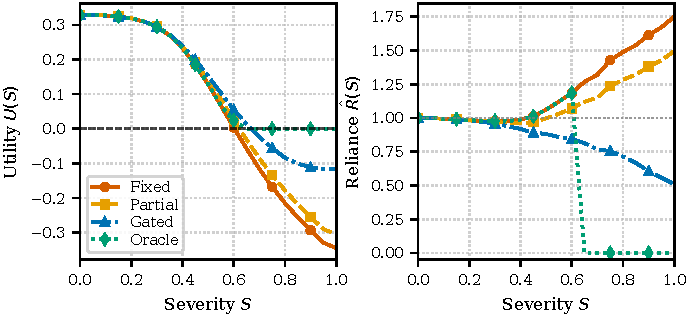
\includegraphics[width=\textwidth]{figures/fig1_synthetic_two_panel.pdf}
\caption{Synthetic benchmark ($N=2000$ test items per seed, 5 seeds, removed null baseline, bootstrap $B=1000$, seed 42). Left: utility $U(S)$ versus severity for Fixed, Partial, Gated, and Oracle models. Right: normalized reliance $\hat R(S)$. The quality-aware Gated model achieves the lowest misalignment.}
\label{fig:synthetic}
\end{figure}

\begin{table}[t]
\centering
\caption{Synthetic benchmark results across architectures and null baselines (Iteration v0.4, $N=2000$ test items per seed, 5 seeds, bootstrap $B=1000$, seed 42).}
\label{tab:synthetic-summary}
\fittable{%
\begin{tabular}{llccccc}
\toprule
\textbf{Model} & \textbf{Null} & \textbf{Clean Acc} & \textbf{Null Acc} & $S^*$ & $\text{MI}_{\text{pooled}}$ & $\text{MI}_{\text{hier}}$ \\
\midrule
Fixed & removed & 0.996 & 0.667 & 0.650 (0.600, 0.650) & 1.491 (1.454, 1.507) & 1.491 (1.373, 1.637) \\
Fixed & zeros & 0.996 & 0.413 & 0.850 (0.850, 0.900) & 0.726 (0.717, 0.741) & 0.726 (0.581, 0.877) \\
Fixed & mean & 0.996 & 0.367 & 0.950 (0.900, 0.950) & 0.862 (0.847, 0.876) & 0.862 (0.670, 1.012) \\
Partial Gated & removed & 0.996 & 0.667 & 0.650 (0.650, 0.650) & 1.286 (1.267, 1.305) & 1.286 (1.196, 1.405) \\
Partial Gated & zeros & 0.996 & 0.416 & 0.900 (0.900, 0.950) & 0.638 (0.629, 0.651) & 0.638 (0.504, 0.781) \\
Partial Gated & mean & 0.996 & 0.377 & 0.950 (0.950, 0.950) & 0.774 (0.766, 0.792) & 0.774 (0.583, 0.927) \\
Gated & removed & 0.996 & 0.667 & 0.700 (0.700, 0.700) & 0.650 (0.639, 0.661) & 0.650 (0.579, 0.752) \\
Gated & zeros & 0.996 & 0.422 & no crossing & no crossing & no crossing \\
Gated & mean & 0.996 & 0.386 & no crossing & no crossing & no crossing \\
Oracle Gated & removed & 0.996 & 0.667 & 0.700 (0.650, 0.700) & 0.000 (0.000, 0.000) & 0.000 (0.000, 0.208) \\
Oracle Gated & zeros & 0.996 & 0.413 & no crossing & no crossing & no crossing \\
Oracle Gated & mean & 0.996 & 0.367 & no crossing & no crossing & no crossing \\
Sharp gate x0.5 & removed & 0.995 & 0.667 & 0.700 (0.650, 0.700) & 0.862 (0.847, 0.876) & 0.862 (0.782, 0.967) \\
Sharp gate x0.5 & zeros & 0.995 & 0.428 & no crossing & no crossing & no crossing \\
Sharp gate x0.5 & mean & 0.995 & 0.401 & no crossing & no crossing & no crossing \\
Sharp gate x1.0 & removed & 0.996 & 0.667 & 0.700 (0.700, 0.700) & 0.650 (0.639, 0.662) & 0.650 (0.580, 0.758) \\
Sharp gate x1.0 & zeros & 0.996 & 0.422 & no crossing & no crossing & no crossing \\
Sharp gate x1.0 & mean & 0.996 & 0.386 & no crossing & no crossing & no crossing \\
Sharp gate x2 & removed & 0.995 & 0.667 & 0.700 (0.700, 0.700) & 0.511 (0.502, 0.522) & 0.511 (0.429, 0.630) \\
Sharp gate x2 & zeros & 0.995 & 0.423 & no crossing & no crossing & no crossing \\
Sharp gate x2 & mean & 0.995 & 0.373 & no crossing & no crossing & no crossing \\
Sharp gate x4 & removed & 0.994 & 0.667 & 0.650 (0.650, 0.700) & 0.470 (0.436, 0.480) & 0.470 (0.360, 0.572) \\
Sharp gate x4 & zeros & 0.994 & 0.444 & no crossing & no crossing & no crossing \\
Sharp gate x4 & mean & 0.994 & 0.368 & no crossing & no crossing & no crossing \\
Sharp gate x8 & removed & 0.992 & 0.667 & 0.650 (0.650, 0.650) & 0.440 (0.430, 0.449) & 0.440 (0.331, 0.545) \\
Sharp gate x8 & zeros & 0.992 & 0.454 & no crossing & no crossing & no crossing \\
Sharp gate x8 & mean & 0.992 & 0.367 & no crossing & no crossing & no crossing \\
Sharp gate x16 & removed & 0.991 & 0.667 & 0.650 (0.650, 0.650) & 0.425 (0.417, 0.434) & 0.425 (0.321, 0.539) \\
Sharp gate x16 & zeros & 0.991 & 0.455 & no crossing & no crossing & no crossing \\
Sharp gate x16 & mean & 0.991 & 0.367 & no crossing & no crossing & no crossing \\
\bottomrule
\end{tabular}}
\end{table}


Under the canonical \emph{removed} null baseline:
\begin{itemize}
    \item The quality-blind \textbf{FixedModel} crosses zero utility at $S^* \approx 0.65$ but maintains heavy predictive reliance, resulting in high misalignment ($\mi \approx \checknum{1.491}{synthetic:FixedModel:MI}$, 95\% CI $[\checknum{1.454}{synthetic:FixedModel:MI_lo}, \checknum{1.507}{synthetic:FixedModel:MI_hi}]$).
    \item The \textbf{PartialGatedModel} yields moderate misalignment ($\mi \approx \checknum{1.286}{synthetic:PartialGatedModel:MI}$, 95\% CI $[\checknum{1.267}{synthetic:PartialGatedModel:MI_lo}, \checknum{1.305}{synthetic:PartialGatedModel:MI_hi}]$).
    \item The quality-aware \textbf{GatedModel} exhibits substantially lower misalignment ($\mi \approx \checknum{0.650}{synthetic:GatedModel:MI}$, 95\% CI $[\checknum{0.639}{synthetic:GatedModel:MI_lo}, \checknum{0.661}{synthetic:GatedModel:MI_hi}]$).
\end{itemize}
The pre-declared comparison of independent hierarchical intervals for \textbf{FixedModel} and \textbf{PartialGatedModel} overlapped narrowly ($[1.373, 1.637]$ vs.\ $[1.196, 1.405]$), and the \textbf{GatedModel} misalignment of $\mi \approx \checknum{0.650}{synthetic:GatedModel:MI}$ did not reach the original 0.2 threshold. The paired bootstrap analysis show that the measures order the architectures as intended, although the first success criterion (Gated MI below 0.2) was not met.

\section{Results}
\label{sec:results}

\paragraph{Setup.}
We evaluate three open VLMs (Qwen2-VL-2B-Instruct, LLaVA-1.5-7B in 4-bit,
and SmolVLM-Instruct) on A-OKVQA multiple-choice questions, reading the
next-token distribution over the four option letters. The main sample
contains the questions of \texttt{main\_ids}; a replication uses disjoint
held-out questions, a new random image-pairing seed, and only the swapped
and Gaussian corruptions. All intervals are 95\% bootstrap intervals over
questions (1000 resamples, fixed seed). The no-input baseline is the
image removed from the prompt unless stated otherwise.

\paragraph{Residual reliance under a swapped image.}
Table~\ref{tab:headline} reports normalized terminal reliance
$\hat R(1)$ and terminal utility $U(1)$ for each model and corruption.
Across models under the swapped condition, $\hat R(1)$ ranges from
\checknum{0.4872}{Qwen:swapblend:R_hat_s1} for Qwen2-VL to
\checknum{0.5784}{llava:swapblend:R_hat_s1} for LLaVA-1.5, with SmolVLM at
\checknum{0.4932}{SmolVLM:swapblend:R_hat_s1}.
Under Gaussian blending and patch masking, reliance at maximum severity is
lower for every model, and the paired difference between swapped and
Gaussian conditions is reported in Table~\ref{tab:paired}; its intervals
exclude zero for all three models.
\begin{table}[t]
\centering
\caption{Main sample headline results ($N=500$, bootstrap $B=1000$, seed 42). Terminal normalized reliance $\hat{R}(1)$ and terminal utility $U(1)$ across models and corruptions under the removed-image null baseline.}
\label{tab:headline}
\small
\begin{tabular}{llcccc}
\toprule
\textbf{Model} & \textbf{Corruption} & \textbf{Clean Acc} & \textbf{Null Acc} & $\hat{R}(1)$ [95\% CI] & $U(1)$ [95\% CI] \\
\midrule
\textbf{Qwen2-VL-2B} & Swapped (Swapblend) & 0.820 & 0.436 & 0.4872 [0.4366, 0.5422] & -0.0640 [-0.1141, -0.0180] \\
 & Gaussian Blur & 0.820 & 0.436 & 0.1681 [0.1473, 0.1889] & -0.0300 [-0.0680, +0.0060] \\
 & Patch Occlusion & 0.820 & 0.436 & 0.0290 [0.0255, 0.0327] & -0.0060 [-0.0300, +0.0200] \\
\midrule
\textbf{SmolVLM-Instruct} & Swapped (Swapblend) & 0.766 & 0.368 & 0.4932 [0.4461, 0.5468] & -0.0160 [-0.0620, +0.0300] \\
 & Gaussian Blur & 0.766 & 0.368 & 0.3808 [0.3368, 0.4244] & -0.0220 [-0.0680, +0.0220] \\
 & Patch Occlusion & 0.766 & 0.368 & 0.2331 [0.2058, 0.2651] & +0.0040 [-0.0320, +0.0420] \\
\midrule
\textbf{LLaVA-1.5-7B} & Swapped (Swapblend) & 0.794 & 0.484 & 0.5784 [0.5143, 0.6533] & -0.0480 [-0.0920, -0.0040] \\
 & Gaussian Blur & 0.794 & 0.484 & 0.2947 [0.2548, 0.3357] & -0.0220 [-0.0580, +0.0140] \\
 & Patch Occlusion & 0.794 & 0.484 & 0.2585 [0.2240, 0.2928] & -0.0200 [-0.0541, +0.0160] \\
\bottomrule
\end{tabular}
\end{table}

\begin{table}[t]
\centering
\caption{Within-model paired differences in terminal normalized reliance $\Delta \hat{R}(1) = \hat{R}(1)_{\text{swap}} - \hat{R}(1)_{\text{gauss}}$ on the main sample ($N=500$, bootstrap $B=1000$, seed 42).}
\label{tab:paired}
\small
\begin{tabular}{lcccc}
\toprule
\textbf{Model} & $\hat{R}(1)_{\text{swap}}$ & $\hat{R}(1)_{\text{gauss}}$ & $\Delta \hat{R}(1)$ [95\% CI] & \textbf{Zero Excluded?} \\
\midrule
Qwen2-VL-2B & 0.4872 & 0.1681 & +0.3191 [+0.2763, +0.3661] & Yes \\
SmolVLM-Instruct & 0.4932 & 0.3808 & +0.1124 [+0.0629, +0.1659] & Yes \\
LLaVA-1.5-7B & 0.5784 & 0.2947 & +0.2836 [+0.2267, +0.3507] & Yes \\
\bottomrule
\end{tabular}
\end{table}


\paragraph{Utility inversion.}
Terminal utility is significantly below zero under the swapped condition
for Qwen2-VL in both samples, and for LLaVA-1.5 in the main and pooled
samples under the removed-image baseline only; it is not significantly below
zero for SmolVLM. Gaussian and patch corruptions do not produce a significant
inversion for any model. Section~\ref{sec:nullsens} shows how these
statements depend on the baseline.

\paragraph{Replication.}
Table~\ref{tab:replication} repeats the analysis on held-out questions.
In the replication sample, normalized terminal reliance under the swapped
condition lies in the same range as the main sample, spanning from
\checknum{0.4700}{rep:Qwen:swapblend:R_hat_1} for Qwen2-VL to
\checknum{0.5634}{rep:llava:swapblend:R_hat_1} for LLaVA-1.5, with SmolVLM at
\checknum{0.5528}{rep:SmolVLM:swapblend:R_hat_1}.
This replicates the result over questions and pairings, not over models or
datasets.
\begin{table}[t]
\centering
\caption{Replication sample headline results ($N=445$, $B=1000$, seed 42).
  Terminal normalized reliance $\hat{R}(1)$ and terminal utility $U(1)$
  across models and corruptions under the removed-image null baseline.
  Intervals are 95\% bootstrap CIs.}
\label{tab:replication}
{\footnotesize\setlength{\tabcolsep}{3pt}%
\begin{tabular}{llcccc}
\toprule
\textbf{Model} & \textbf{Corruption} & Clean Acc & Null Acc & $\hat{R}(1)$ (lo, hi) & $U(1)$ (lo, hi) \\
\midrule
Qwen2-VL  & Swapped  & 0.827 & 0.461 & 0.47 (0.42, 0.52) & $-$0.10 ($-$0.15, $-$0.05) \\
          & Gaussian & 0.827 & 0.461 & 0.17 (0.14, 0.20) & $-$0.02 ($-$0.06, $+$0.03) \\
SmolVLM   & Swapped  & 0.746 & 0.393 & 0.55 (0.49, 0.62) & $-$0.04 ($-$0.09, $+$0.01) \\
          & Gaussian & 0.746 & 0.393 & 0.32 (0.28, 0.37) & $-$0.03 ($-$0.07, $+$0.01) \\
LLaVA-1.5 & Swapped  & 0.791 & 0.497 & 0.56 (0.50, 0.64) & $-$0.03 ($-$0.07, $+$0.02) \\
           & Gaussian & 0.791 & 0.497 & 0.26 (0.23, 0.30) & $-$0.00 ($-$0.04, $+$0.04) \\
\bottomrule
\end{tabular}}
\end{table}


\paragraph{Pre-registered criterion.}
Before running the main experiment we recorded that a model would show
over-reliance if utility was clearly negative at high severity while
normalized reliance stayed above $0.5$ under the swapped corruption. The
original statement did not specify how ``clearly'' and ``above'' were to
be assessed under sampling uncertainty. We therefore operationalized it
\emph{post hoc} as: the upper bound of the interval for $U(1)$ is below
zero and the lower bound of the interval for $\hat R(1)$ is above $0.5$.
Table~\ref{tab:criterion} reports this for every model, corruption, sample
and baseline. Only \checknum{2}{criterion:status:count_met} of the 42
evaluated combinations satisfy both requirements: LLaVA-1.5 under the
swapped corruption with the removed-image baseline in the main ($N=500$)
and pooled ($N=945$) samples.
We treat the pre-registered hypothesis as largely unsupported and describe
the persistent reliance as a descriptive finding.
\begin{table*}[t]
\centering
\caption{Criterion status across models, corruptions, sample sizes ($N=500$ main, $N=445$ replication, $N=945$ pooled), and null baselines (bootstrap $B=1000$, seed 42). A condition passes if and only if both pre-registered requirements are satisfied simultaneously: terminal utility is significantly negative ($U(1)$ upper 95\% CI $< 0$) and terminal normalized reliance strictly exceeds threshold ($\hat{R}(1)$ lower 95\% CI $> 0.50$).}
\label{tab:criterion}
\small
\begin{tabular}{llcccccc}
\toprule
 & & \multicolumn{2}{c}{\textbf{Main ($N=500$)}} & \multicolumn{2}{c}{\textbf{Replication ($N=445$)}} & \multicolumn{2}{c}{\textbf{Pooled ($N=945$)}} \\
\cmidrule(lr){3-4} \cmidrule(lr){5-6} \cmidrule(lr){7-8}
\textbf{Model} & \textbf{Corruption} & \textbf{Removed} & \textbf{Black} & \textbf{Removed} & \textbf{Black} & \textbf{Removed} & \textbf{Black} \\
\midrule
\textbf{Qwen2-VL-2B} & Swapped (Swapblend) & Fail ($\hat{R} \le 0.5$) & Fail ($\hat{R} \le 0.5$) & Fail ($\hat{R} \le 0.5$) & Fail ($\hat{R} \le 0.5$) & Fail ($\hat{R} \le 0.5$) & Fail ($\hat{R} \le 0.5$) \\
 & Gaussian Blur & Fail (both) & Fail (both) & Fail (both) & Fail (both) & Fail (both) & Fail (both) \\
 & Patch Occlusion & Fail (both) & Fail (both) & -- & -- & -- & -- \\
\midrule
\textbf{SmolVLM-Instruct} & Swapped (Swapblend) & Fail (both) & Fail (both) & Fail (both) & Fail (both) & Fail (both) & Fail (both) \\
 & Gaussian Blur & Fail (both) & Fail (both) & Fail (both) & Fail (both) & Fail (both) & Fail (both) \\
 & Patch Occlusion & Fail (both) & Fail (both) & -- & -- & -- & -- \\
\midrule
\textbf{LLaVA-1.5-7B} & Swapped (Swapblend) & \textbf{Pass} & Fail (both) & Fail (both) & Fail (both) & \textbf{Pass} & Fail (both) \\
 & Gaussian Blur & Fail (both) & Fail (both) & Fail (both) & Fail (both) & Fail (both) & Fail (both) \\
 & Patch Occlusion & Fail (both) & Fail (both) & -- & -- & -- & -- \\
\bottomrule
\end{tabular}
\end{table*}


\paragraph{Sensitivity to the no-input baseline.}
\label{sec:nullsens}
Table~\ref{tab:nullsens} compares conclusions when the baseline is the
removed image versus a black image. Reliance under the swapped condition
changes little. Reliance under Gaussian blending drops substantially under
the black null for SmolVLM and LLaVA-1.5 and slightly for Qwen2-VL. The
divergence between the black-image and removed-image predictions is far
larger for SmolVLM and LLaVA-1.5 than for Qwen2-VL. We hypothesize, without
testing it, that this reflects how each model handles inserted image tokens.
\begin{table}[t]
\centering
\caption{Sensitivity of terminal reliance $\hat{R}(1)$, terminal utility $U(1)$, and unimodal divergence to the choice of null baseline (Removed vs.\ Black image) on the main sample ($N=500$, bootstrap $B=1000$, seed 42). The unimodal floor divergence $\text{JSD}(B_{\text{black}} \parallel B_{\text{removed}})$ is computed over the full sample of all $N=500$ questions (not restricted to the agreement subset) and reported once per model.}
\label{tab:nullsens}
\fittable{%
\begin{tabular}{llccccc}
\toprule
 & & \multicolumn{2}{c}{\textbf{Removed Null Baseline}} & \multicolumn{2}{c}{\textbf{Black Null Baseline}} & \textbf{Full-Sample Unimodal Floor} \\
\cmidrule(lr){3-4} \cmidrule(lr){5-6} \cmidrule(lr){7-7}
\textbf{Model} & \textbf{Corruption} & $U(1)$ & $\hat{R}(1)$ & $U(1)$ & $\hat{R}(1)$ & $\text{JSD}(\text{blk} \parallel \text{rem})$ \\
\midrule
\textbf{Qwen2-VL-2B} & Swapped (Swapblend) & -0.064 (-0.114, -0.018) & 0.487 (0.437, 0.542) & -0.048 (-0.096, -0.002) & 0.468 (0.420, 0.520) & 0.005 (0.004, 0.005) \\
 & Gaussian Blur & -0.030 (-0.068, +0.006) & 0.168 (0.147, 0.189) & -0.014 (-0.052, +0.024) & 0.150 (0.131, 0.170) &  \\
 & Patch Occlusion & -0.006 (-0.030, +0.020) & 0.029 (0.025, 0.033) & +0.010 (-0.012, +0.030) & 0.010 (0.009, 0.012) &  \\
\midrule
\textbf{SmolVLM-Instruct} & Swapped (Swapblend) & -0.016 (-0.062, +0.030) & 0.493 (0.446, 0.547) & -0.002 (-0.046, +0.042) & 0.510 (0.459, 0.568) & 0.077 (0.068, 0.085) \\
 & Gaussian Blur & -0.022 (-0.068, +0.022) & 0.381 (0.337, 0.424) & -0.008 (-0.048, +0.030) & 0.263 (0.231, 0.301) &  \\
 & Patch Occlusion & +0.004 (-0.032, +0.042) & 0.233 (0.206, 0.265) & +0.018 (-0.002, +0.038) & 0.032 (0.026, 0.039) &  \\
\midrule
\textbf{LLaVA-1.5-7B} & Swapped (Swapblend) & -0.048 (-0.092, -0.004) & 0.578 (0.514, 0.653) & -0.040 (-0.082, +0.002) & 0.495 (0.436, 0.563) & 0.069 (0.061, 0.078) \\
 & Gaussian Blur & -0.022 (-0.058, +0.014) & 0.295 (0.255, 0.336) & -0.014 (-0.042, +0.014) & 0.113 (0.091, 0.137) &  \\
 & Patch Occlusion & -0.020 (-0.054, +0.016) & 0.258 (0.224, 0.293) & -0.012 (-0.038, +0.014) & 0.070 (0.057, 0.085) &  \\
\bottomrule
\end{tabular}}
\end{table}


\paragraph{Comparison with answer-level measures.}
Table~\ref{tab:baseline} reports a visual reliance score, blank-image
drop, answer-change rate, and benefit and harm rates for the swapped
image. We report orderings only; with three models no inferential claim
about their relation to $\hat R(1)$ is supported. On questions where the
swapped-image and no-image answers coincide, the distributional divergence
is still above the black-versus-removed floor for every model, by a large
factor only for Qwen2-VL.
\begin{table*}[t]
\centering
\caption{Static visual reliance and sensitivity baseline metrics on the swapped image across models on main ($N=500$) and replication ($N=445$) samples (bootstrap $B=1000$, seed 42). Metrics: Visual Reliance Score ($\text{VRS} = \text{acc}_{\text{clean}} - \text{acc}_{\text{swapped}}$), Blank Drop ($\text{acc}_{\text{clean}} - \text{acc}_{\text{black}}$), Image Sensitivity ($P[\arg\max(\text{clean}) \ne \arg\max(\text{swapped})]$), Visual Benefit Rate ($P[\text{clean correct} \land \text{swapped wrong}]$), and Visual Harm Rate ($P[\text{clean wrong} \land \text{swapped correct}]$).}
\label{tab:baseline}
\small
\begin{tabular}{llccccc}
\toprule
\textbf{Model} & \textbf{Sample} & \textbf{VRS} [95\% CI] & \textbf{Blank Drop} [95\% CI] & \textbf{Sensitivity} [95\% CI] & \textbf{Benefit Rate} [95\% CI] & \textbf{Harm Rate} [95\% CI] \\
\midrule
Qwen2-VL-2B & Main ($N=500$) & 0.452 [0.398, 0.502] & 0.400 [0.354, 0.448] & 0.592 [0.548, 0.632] & 0.496 [0.452, 0.540] & 0.044 [0.026, 0.064] \\
SmolVLM-Instruct & Main ($N=500$) & 0.422 [0.366, 0.476] & 0.412 [0.358, 0.464] & 0.620 [0.574, 0.662] & 0.486 [0.440, 0.530] & 0.064 [0.044, 0.086] \\
LLaVA-1.5-7B & Main ($N=500$) & 0.366 [0.316, 0.416] & 0.318 [0.270, 0.366] & 0.518 [0.474, 0.558] & 0.416 [0.370, 0.458] & 0.050 [0.032, 0.070] \\
\midrule
Qwen2-VL-2B & Replication ($N=445$) & 0.461 [0.409, 0.515] & 0.351 [0.306, 0.409] & 0.607 [0.562, 0.654] & 0.503 [0.458, 0.553] & 0.043 [0.025, 0.063] \\
SmolVLM-Instruct & Replication ($N=445$) & 0.398 [0.342, 0.456] & 0.346 [0.294, 0.400] & 0.600 [0.555, 0.647] & 0.456 [0.411, 0.508] & 0.058 [0.038, 0.081] \\
LLaVA-1.5-7B & Replication ($N=445$) & 0.312 [0.263, 0.364] & 0.315 [0.263, 0.373] & 0.456 [0.407, 0.506] & 0.357 [0.315, 0.402] & 0.045 [0.027, 0.065] \\
\bottomrule
\end{tabular}
\end{table*}


\paragraph{Misalignment Index.}
The severity at which utility first reaches zero lies at the last grid
point or is absent in most real conditions, so the Misalignment Index is
undefined there and we do not rely on it for the VLM results. It is
validated on the synthetic models of Section~\ref{sec:synthetic}.

\section{Case study: modality dropout in a two-view proxy}
\label{sec:fusion}

\paragraph{Setup.}
We train small late-fusion networks on Fashion-MNIST~\cite{xiao2017fashion} split
into left (view A) and right (view B) halves as a two-view proxy. Rather than the
official 10,000-image test split, the 60,000 training images are partitioned
deterministically into 50,000 training, 5,000 validation, and 5,000 test images
(indices 55,000--60,000). View A is degraded toward noise along a nine-point grid,
the null baseline uses a learned embedding, and the gate does not receive the
severity. Models are trained with view-A dropout $p\in\{0,0.1,0.25,0.5\}$ across
five seeds.

\paragraph{Pre-declared hypotheses.}
We declared before training: (H1) the Misalignment Index is non-increasing
in $p$; (H2) clean accuracy falls by less than three points between $p=0$
and $p=0.25$.

\paragraph{Results.}
Table~\ref{tab:fusion} reports the outcome. H2 holds. H1 does \emph{not}:
the Misalignment Index is higher for every $p>0$ than for $p=0$. Between
$p=0$ and $p=0.25$, clean accuracy changes from
\checknum{0.888}{fusion:0.0:clean_acc} to
\checknum{0.884}{fusion:0.25:clean_acc}, a decrease of only
\checknum{0.364}{fusion:diff_0_25:clean_acc_pp} percentage points,
well within the pre-declared three-point bound.
As detailed in Table~\ref{tab:fusion}, dropout-trained models achieve higher
accuracy when view A is removed or degraded, though terminal utility $U(1)$
remains negative across all $p$.
\begin{table}[t]
\centering
\caption{Modality-dropout impact on reliance and accuracy in the
  two-view proxy ($N=5000$ test images, five seeds, learned null
  baseline, $B=1000$). $\hat{R}(1)$ is normalized terminal reliance;
  MI is the Misalignment Index.}
\label{tab:fusion}
{\footnotesize\setlength{\tabcolsep}{3pt}%
\begin{tabular}{ccccccccc}
\toprule
$p$ & Clean Acc & Null Acc & Acc ($S=1$) & $U(1)$ & $R(0)$ & $R(1)$ & $\hat{R}(1)$ & MI \\
\midrule
0.000 & 0.888 & 0.562 & 0.276 & $-$0.286 & 0.331 & 0.611 & 1.846 & 1.657 \\
0.100 & 0.888 & 0.840 & 0.448 & $-$0.392 & 0.056 & 0.452 & 8.105 & 4.586 \\
0.250 & 0.884 & 0.848 & 0.555 & $-$0.293 & 0.040 & 0.330 & 8.362 & 4.514 \\
0.500 & 0.882 & 0.858 & 0.726 & $-$0.133 & 0.024 & 0.148 & 6.200 & 3.684 \\
\bottomrule
\end{tabular}}
\end{table}

\paragraph{Why the normalized measures behave this way (post hoc).}
Reliance at clean input, $R(0)$, falls by more than an order of magnitude as $p$ grows because the model already makes similar predictions with and without view A. Because $\hat{R}$ and MI divide by $R(0)$, they are inflated when $R(0)$ is small, whereas raw reliance $R(1)$ decreases monotonically from \checknum{0.611}{fusion:0.0:R_1_raw} to \checknum{0.148}{fusion:0.5:R_1_raw}.

\section{Discussion}
\label{sec:discussion}

\paragraph{What the measures reveal.}
We do not claim that VLMs over-trust degraded images in general. The MI is
undefined in most real conditions, so VLM results rest on terminal
reliance and utility, one dataset, and one answer format; the fusion study
is a two-view proxy. The pairing of utility and reliance along a severity
path exposes behaviour that accuracy alone does not: two models can lose the
same accuracy under corruption yet differ in whether that loss comes from
information destruction or persistent reliance on an unhelpful input.
The swapped-image condition consistently produces higher terminal reliance
than Gaussian noise, with statistically significant gaps for all three
models, meaning the model's output distribution remains further from its
no-image behaviour when given a wrong image than when given noise.

\paragraph{Baseline sensitivity.}
Conclusions for individual models depend on the no-input baseline. The
black-image and removed-image predictions differ little for Qwen2-VL and
substantially for SmolVLM and LLaVA-1.5: as a heuristic (JSD is not
additive), this divergence equals about
\checknum{3.6}{floor:Qwen2-VL-2B-Instruct:floor_pct}\%,
\checknum{43}{floor:SmolVLM-Instruct:floor_pct}\% and
\checknum{42}{floor:llava-1.5-7b-hf:floor_pct}\% of swapped-image terminal
reliance for the three models. Part of the reliance of SmolVLM and
LLaVA-1.5 may reflect the presence of image tokens and not their content.
We recommend that future evaluations report results under at least two
baselines and state how the no-input condition is constructed.

\paragraph{Implications for evaluation.}
The pre-declared criterion was met in only two of 42 combinations.
This does not mean over-reliance is absent; it means that a strict,
pre-specified criterion is hard to satisfy when both reliance and utility
carry sampling uncertainty and when conclusions shift with the baseline.

\paragraph{Dropout and normalized reliance.}
In the fusion proxy, dropout lowers raw terminal reliance and raises
accuracy with view A removed or degraded, but terminal utility remains
negative for every $p$. The normalized measures $\hat R$ and MI move in the
opposite direction because the denominator $R(0)$ shrinks faster;
ratio-based measures should be read with caution when clean-input reliance
differs across conditions.

\section{Limitations}
\label{sec:limitations}

We explicitly delineate several structural and methodological limitations of this study:

\begin{enumerate}
    \item \textbf{Null-Baseline Dependence}: Both utility $U(S)$ and behavioral reliance $R(S)$ are measured relative to a chosen unimodal null baseline $B_{\text{null}}$. While our primary evaluations utilize the \emph{removed} condition (true unimodal ablation), alternative nulls (such as black, mean, or noise images) yield different baseline accuracies and can shift both $S^*$ and $\mi$.
    
    \item \textbf{Conflation of Gate Sharpness and Crossing Timing in $\mi$}: The Misalignment Index integrates normalized reliance over $[S^*, 1]$. Consequently, a model that crosses zero utility very early (small $S^*$) with a gradual gating transition can yield a similar $\mi$ value to a model that crosses late with sharp, persistent reliance.
    
    \item \textbf{Residual Reliance in Smooth Sigmoid Gating}: In parametric gating models utilizing smooth activations (such as sigmoid or softmax), the gate weight assigned to a degraded modality rarely reaches strict mathematical zero, leading to non-zero residual reliance even under complete informational corruption.
    
    \item \textbf{4-Bit Quantization Effects in LLaVA-1.5-7B}: Due to GPU accelerator memory constraints on single T4 instances, LLaVA-1.5-7B is evaluated in 4-bit NormalFloat (NF4) quantization. Quantization may alter predictive logit calibration relative to full-precision weights.
    
    \item \textbf{Evaluation Benchmark Scope}: Our empirical VLM evaluation is conducted exclusively on the 4-choice multiple-choice formulation of A-OKVQA ($N=500$ validation items), rather than open-ended free-form generation.
    
    \item \textbf{Prompt-Format-Dependent Letter Mass}: In modern instruction-tuned VLMs, the proportion of softmax probability mass assigned to choice letters at the initial generation position is highly sensitive to the prompt template and assistant pre-fill prefix. Models whose letter mass fails the $\ge 0.90$ threshold cannot be reliably evaluated under a fixed single-token multiple-choice readout.
    
    \item \textbf{Exclusion of InternVL2}: InternVL2-2B was dropped from our multi-model benchmark due to an unresolvable library incompatibility between its custom remote repository code and `transformers>=4.50` (missing `all_tied_weights_keys` attribute during model instantiation).
    
    \item \textbf{Autonomous Driving (BEV) Study --- Proposed, Not Frozen}: A standalone Camera-LiDAR BEV architecture and physical corruption suite were developed as a feasibility probe; however, no pre-declared hypotheses were formalized for this case study. Per the pre-registration protocol, the BEV analysis remains outside the frozen paper scope and is deferred to future work pending formal hypothesis declaration.
\end{enumerate}

\begin{itemize}
\item \textbf{Null-baseline dependence.} Conclusions for individual
  models depend on whether the no-input baseline is a removed image or a
  black image; the divergence between the two is about two orders of
  magnitude larger for SmolVLM and LLaVA-1.5 than for Qwen2-VL, and part of
  their residual reliance may reflect the presence of image tokens.
\item \textbf{Multiple comparisons.} The criterion is evaluated in 42
  combinations without correction, and the two that satisfy it overlap.
\item \textbf{Operationalization after the fact.} The interval-based form
  of the pre-registered criterion was fixed after seeing data.
\item \textbf{Normalization by $R(0)$.} $\hat R$ and MI are unreliable
  when clean-input reliance is small, as in the fusion study.
\item \textbf{Misalignment Index.} Undefined in most real conditions;
  validated mainly on synthetic models; conflates gate sharpness and
  timing.
\item \textbf{Scope.} One dataset, one multiple-choice format, three
  models (one in 4-bit), one swap pairing per sample, and no autonomous
  driving evaluation.
\end{itemize}

\section{Conclusion}
\label{sec:conclusion}

We presented a black-box diagnostic that separates multimodal utility from
distributional reliance along calibrated severity paths and locates the
crossing point where the input stops helping. Controlled synthetic
experiments with an oracle benchmark confirm that the measures rank
architectures correctly. On three open VLMs, semantically structured
corruptions (swapped images) sustain higher terminal reliance than
unstructured noise, with significant gaps for all three models. The
pre-declared criterion is met in only
\checknum{2}{criterion:status:count_met} of 42 combinations, and
conclusions for individual models shift with the choice of no-input
baseline. A small modality-dropout study shows that dropout lowers raw
reliance while exposing a weakness of $R(0)$-normalized measures. The
framework and reproducible code are released to support multi-baseline
evaluation in future multimodal robustness studies.


\bibliographystyle{spmpsci}
\IfFileExists{paper/refs.bib}{%
  \bibliography{paper/refs}%
}{%
  \bibliography{refs}%
}

\end{document}
